\documentclass[notitlepage,a4paper,11pt]{article}

\usepackage{subcaption}
\usepackage[english]{babel}
\usepackage{blindtext}
\usepackage{microtype}
\usepackage{wrapfig}
\usepackage{graphicx} %inserting graphics
\usepackage{wrapfig}  %wrapping text around image
\usepackage{enumitem} %for lists
\usepackage{fancyhdr} %fancy headers
\usepackage{amsmath} %for maths
\usepackage{amssymb}
\usepackage{index} %for indexes
\usepackage{apacite} %APA referencing
\usepackage[ruled,vlined]{algorithm2e}

\newcommand{\R}{\mathbb{R}}
\pagenumbering{roman} 
  
\DeclareMathOperator{\E}{\mathbb{E}}
\usepackage[a4paper]{geometry}
\graphicspath{ {./} }
\makeindex

\geometry{a4paper, total={170mm, 257mm}, left=20mm, top=20mm}

\begin{document}

\title{\textbf{Final Report\\
	\large{Hierarchical Deep Reinforcement Learning in Super Mario}}}

\author{660050748}
\date{April 29th, 2020}
\maketitle

\begin{abstract}
 
\end{abstract}


\vspace*{\fill}
\textit{I certify that all material in this dissertation which is not my own work has been identified.}

\fancyhf{}
\fancyhead[LE]{\leftmark}
\fancyhead[RO]{\rightmark}

\fancyfoot[LE,RO]{\thepage}
\pagebreak

\tableofcontents1

\pagebreak
\pagenumbering{arabic}
\section{Introduction}
Reinforcement Learning is a field of Machine Learning where autonomous agents learn how to act optimally and maximise a reward within a given environment. Throughout the last decade, the field has achieved remarkable successes and gained significant medial and research attention. Algorithms have been shown to outperform the best human players on a wide range of Atari games \cite{DBLP:journals/corr/MnihKSGAWR13}, chess, Shogi and the strategy board game Go \cite{alpha_go}, and even Starcraft \cite{arulkumaran2019alphastar}. Super Mario as a domain is not as popular as the Atari games amongst researchers, making it an interesting choice for testing Reinforcement Learning algorithms.  The goal of this project is to investigate, test, evaluate and compare a number of Reinforcement Learning algorithms on the domain of NES Super Mario. 



\subsection{Motivation}
Reinforcement Learning algorithms come in many flavours, however most do so called \textit{tabula-rasa} (blank-slate) learning. Humans are experts at reusing prior knowledge in new situations, e.g. if you see a ladder in a video game you have never played before, you know that you can climb that ladder because you know what a ladder is. A \textit{tabula-rasa} agent on the other hand will first have to learn concepts a human player already brings to the table. Moreover, even if the agent learns to climb the ladder, it has no concept thereof and will have to relearn it in a new situation. For this reason, contemporary algorithms that play at a superhuman level require absurd amounts of training episodes on powerful hardware. DeepMind's Rainbow architecture \cite{hessel2018rainbow} attains superhuman performance after experiencing 18 million frames, corresponding to 83
hours of Atari gameplay. Distributional RL \cite{bellemare2017distributional} surpasses human
players after 70 million frames in Atari games. If agents were able to abstract away behaviour when learning and reuse already learned information when faced with new situations, the training time could be reduced. Additionally, the agent would be more capable of generalisation.

Introducing the abstraction of behaviour is the research area of Hierarchical Reinforcement Learning. Instead of treating the solution to a Super Mario level purely as a sequence of primitive actions, e.g. pressing left, right, jump etc, Hierarchical Reinforcement Learning breaks down the solution into more abstract learnable chunks. These chunks operate at a higher \textit{temporal abstraction} and act as subgoals for an agent to achieve in the game. Intuitively, this is how a human player would approach the game as well. They would most likely not think in terms of button combinations however, but on a higher level.To finish a level, Mario has to jump ravines, kill Goombas, avoid Fire Bars and climb steps - all of which are further decomposable into arrangements of primitive left, right, jump actions. Recent research \cite{nachum2019does} has shown that using an Hierarchical Approach to learning, results in up to 3 - 5 times fewer interactions with the environment. Thus, Hierarchical Reinforcement Learning comes with potential to alleviate the problem of long training times. 

\subsection{Objectives}
The main objective of this project was to compare 

\section{Theoretical Background}
The following section will provide the theoretical underbody for the different Reinforcement Learning approaches used in this project. 


\subsection{Deep Reinforcement Learning}
Deep Reinforcement Learning combines neural networks with the concepts of traditional Reinforcement Learning and is the contemporary go-to approach. This section will outline the basic concepts of Reinforcement Learning and explain the improvements made by neural networks. The environment in an RL-problem is typically modelled as a Markov-Decision-Process (MDP). It is a discrete stochastic sequential decision process \cite{puterman2014markov} formalised as a 5-part tuple $\langle S, A, T, R, \gamma \rangle$ where:

\begin{itemize}[noitemsep]
	\item $S$ is the state space, i.e. the set of all possible states. For Mario, each pixel configuration is a state.
	\item $A$ is the action space, i.e. the set of all possible actions. For Mario, these are the different left, right, jump etc. actions.
	\item $T : S \times A \times S \to [0,1]$ is a transition function. It gives conditional probabilities for state traversal.
	\item $R : S \times A \times S \to \R$ is a reward function. It gives a real number for state traversal. The reward function used in this project is described in section \ref{reward_function}.
	\item $\gamma$ is a discount factor to prevent infinite rewards.
\end{itemize}
\cite{franccois2018introduction}\\\\
At a given point in time $t$, the agent performs an action $a_t$ in state $s_t$ and observes a reward $r_t$ and a new state $s_{t+1}$. Actions only last a single timestep, e.g. it is not possible to take action $a_t$ and move from state $s_t$ to state $s_{t+5}$. Moving from state $s_t$ to state $s_{t+1}$ is noisy and happens with probability $P(s_t, a_t | s_{t+1})$ as defined by the transition function $T$. While deterministic MDPs exist where the transition function always returns $1$, they are neither applicable to real-world scenarios nor to this project. Which action to perform in a given state is dictated by a policy $\pi$. An optimal policy $\pi^*$ will always prescribe the action which gives the highest expected return of reward for every state in the state space.

\begin{figure}[!htb]
\centering
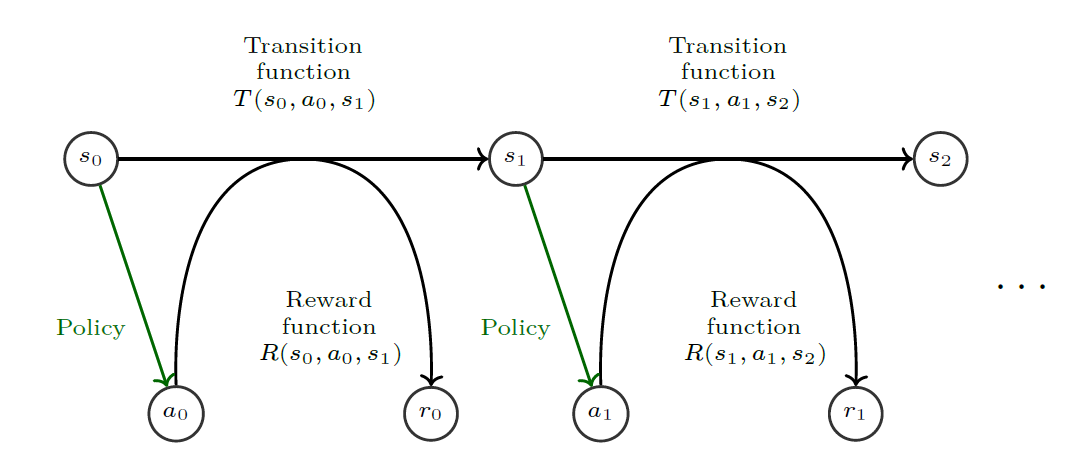
\includegraphics[width=.5\linewidth]{figs/mdp_detail.png}
\caption{Agent takes an action to move to the next state and observe a reward \protect\cite{franccois2018introduction}} \label{fig:2}
\end{figure}

One of the most popular algorithms for learning optimal policies remains Q-learning \cite{watkins1992q}. Each state in the state space has state-action pairs called Q-values. The Q-value $Q(s,a)$ describes the rewards an agent can expect from taking taking action $a$ in state $s$. For instance, if Mario encounters a Goomba in his current state, the Q-value for taking an action running into the Goomba would be lower than the Q-value for taking an action killing the Goomba. The Q-value under a policy $\pi$ is formalised as the expected sum of discounted rewards \textbf{given} state $s$ and action $a$:

\[ 
 Q^\pi(s, a) = \E \left[ \sum_{k=0}^{\infty} \gamma^k R_{t+k+1} \Big| S_t = s, A_t = a \right]
\]

An optimal policy is therefore one which for each state chooses the action associated with the largest Q-value. All an agent has to do in order to learn an optimal policy is the Q function: $Q : S \times A \to \R$. The agent learns by continuously experiencing the environment, updating the Q-values until they converge using the following equation:

\[
	Q(s,a) \gets Q(s,a) + \alpha \left[ R + \gamma \max\limits_{a^\prime} Q(S^\prime, a^\prime) - Q(s,a) \right] 
\]

Whenever an agent takes an action in a state and experiences a reward, the old Q-value needs to be updated to reflect that observation. This is done by adding the experienced reward $R$ for taking action $a$ in state $s$ to the discounted largest Q-value of the next state $Q(S^\prime, a^\prime)$ ($\gamma$ is the discount factor), subtracting the old Q-value, multiplying everything by the learning rate $\alpha$ and adding it to the old Q-value. The learning rate specifies the importance of new information \textit{vis-à-vis} old information. In traditional RL, the Q-function is a lookup table where each entry corresponds to a Q-value. Q-tables quickly become infeasible for complex problems however. For instance, assuming an image size of $84 \times 84$, the RGB Super Mario state space has a size of $(84 \times 84 \times 3)^{256}$. The solution is to replace the lookup table with a neural network. This works because neural networks in essence are universal function approximators. Especially Convolutional Neural Networks have made it possible to identify features in images and map them to outputs, thus reducing the need for a large memory footprint and allowing the application of Reinforcement Learning to high-dimensional problems. 

\subsection{Hierarchical Reinforcement Learning}
Arguably, one of humans' most remarkable abilities is the ability to generalise knowledge \cite{geirhos2018generalisation} across various contexts withstanding input distribution changes. For example, you are able to recognise a door as a door and open it regardless of its colour or material because you abstract away the features which make up the door and generalise it to other doors. While Deep Reinforcement Learning partially alleviates the issue of generalisation \cite{sutton1996generalization}, it remains a substantial issue \cite{van2017hybrid} to date. Reinforcement Learning agents are prone to overspecialise and overfit because they are trained and tested within the same environment \cite{cobbe2018quantifying}. If Mario is trained to solve level \textit{World 1-1}, he only becomes an expert on that particular level. When placed in the next level, he would not perform as well because Mario did not \textbf{learn} any concepts of the world. Instead, he \textbf{remembers} optimal action sequences only applicable to a distinct problem. This is also known as \textit{flat} Reinforcement Learning.

Learning reusable skills is the essence of Hierarchical Reinforcement Learning. It is inspired by the fact that human decision making is \textit{temporally abstract} \cite{sutton1999between} and hierarchically composed. When leaving work to go home, you need to exit the office, however first you need to get up from your chair and take the lift downstairs. The parent task of going home contains multiple subtasks which themselves involve subtasks of their own. By decomposing the overall problem into smaller subproblems, learning is sped up and actions can be reused across the domain. This requires some modification to the MDP used in tradiational Reinforcement Learning. Remember that in \textit{flat} learning, each action $a_t$ only lasts a single timestep. Now, the agent can execute actions lasting multiple timesteps. An action $a_t$ in state $s_t$ can transport the agent to state $s^{\prime}_{t+k}$. The policy $\pi$ is made up of multiple sub-policies, each of which are catering to a specific subset of the state space. 

\begin{figure}[!htb]
\centering
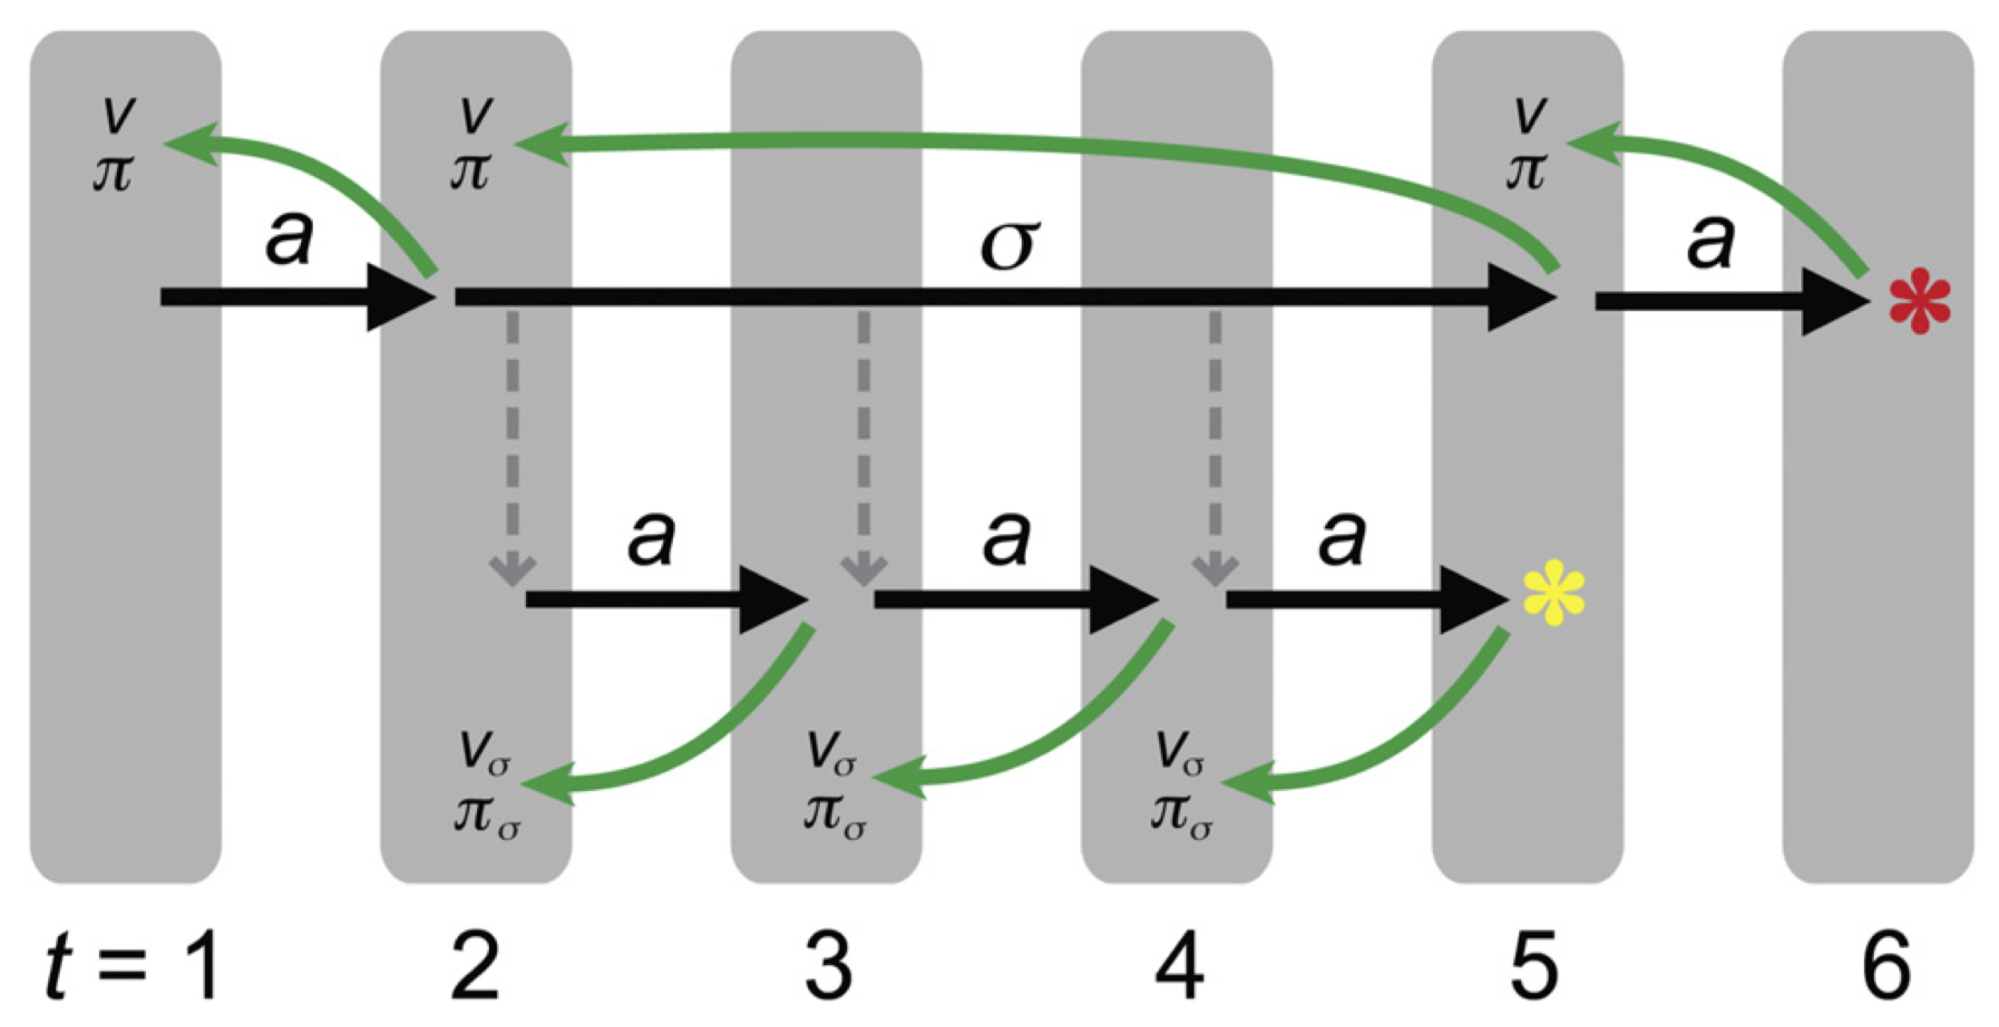
\includegraphics[width=.5\linewidth]{figs/hrl_smdp.png}
\caption{The Hierarchical RL Semi Markov Decision Process \protect\cite{ribas2011neural}} \label{fig:3}
\end{figure}

At timestep $t_1$, the primitive action $a$ is selected and lasts one timestep. At $t_2$, the policy $\pi$ invokes a subpolicy or subtask $\sigma$ which is in charge of selecting primitive actions until $t_5$. Upon termination, the subpolicy returns a reward (yellow asterisk) back to the master policy which incorporates it into the value of the state from where the policy was invoked. 

\subsubsection{Option-Critic}
The following Hierarchical algorithm is an advancement on the Markov-Options framework \cite{sutton1999between} which first introduced a framework for extending the classical one-timestep-action MDP to a multi-timestep-actions Semi MDP (SMDP). In Sutton et. al's work, the options/subpolicies had to be handcrafted for the agent to be able to use them. Additionally, learning these subpolicies comes at a great temporal and spatial expense. The Option-Critic architecture \cite{bacon2017option} not only discovers subpolicies autonomously, but also simultaneously learns the policy over options as well as subpolicies. 

\subsubsection{Feudal Networks}


\section{Specifications and Design}

\subsection{System Requirements}
The following section specifies the requirements to be fulfilled by the system:

\begin{itemize}

	\item \textbf{Super Mario Game Emulator}\\ 
	The Reinforcement Learning agent within the system must have the ability to interact with the Super Mario Bros game environment to obtain information about states, rewards and to perform actions. The Python OpenAI Gym library provides a plugin to play Super Mario, however this plugin does not allow the creation of custom levels (more on custom levels in the next point). Instead, the sytem will use the Mario AI Tenth Anniversary Edition \cite{marioai} framework. Although written in Java, it provides the user with the ability to create their own levels using ASCII art.
	
	\item \textbf{Custom Levels}\\
	Using custom levels means that we can better investigate Mario's generalisation abilities. The agent can learn specific skills in specially designed levels and slowly expand their skillset. This is also the main reason for choosing the Mario AI Tenth Anniversary Edition framework over the OpenAI Gym library. OpenAI Gym only provides the original Super Mario levels and therefore makes the skill stacking with Hierarchical Reinforcement Learning algorithms less transparent.
	
	\item \textbf{Java-Python Bridge}\\
	Because the chosen Super Mario game framework is written in Java and Python is the de facto lingua franca of Reinforcement Learning, the system needs to have a communication bridge between the languages. The system needs to train for longer periods of time, so avoiding unnecessary overhead whereever possible is important. Getting the two languages "as close" as possible to each other is therefore vital. A client-server architecture using HTTP to send JSON is easy to implement, however comes with too much overhead. The Jython \cite{jython} and JPype \cite{jpype} frameworks are directly embedded in the JVM to reduce latency, however they are not as out of the box user friendly. The Py4J \cite{py4j} framework on the other hand uses sockets to communicate with the Java API which leads to a slight performance decrease. Though it is nearly effortless to setup and easy to use which is why it is the best choice for the system.
	
	\item \textbf{Deep Learning Libraries}\\
	Contemporary Reinforcement Learning algorithms rely on Neural Networks to learn behaviour. The system needs to be able to initialise and train neural networks by making use of existing libraries. PyTorch is the most suitable option as it offers a good balance between low-level granularity and easy to use high-level API. Additionally, PyTorch has their own Reinforcement Learning tutorials.
	
	\item \textbf{Preprocessing}\\
	The environment as observed by the Reinforcement Learning agent is a pixel matrix of the current frame of the game. Commonly, frames are cropped and scaled before being passed to the neural network. Cropping removes unnecessary information such as the score and timer counters at the top of the screen. Scaling reduces the complexity of the image and the number of neurons needed in the network. For to reduce latency, cropping and scaling will need to be done on the Java side of the system.
	
	\item \textbf{Monitor Training}\\
	Reinforcement Learning algorithms need to train for anything from several hours to several days. Monitoring this process while it is going on is important because bugs can be caught early on and hyperparameters are more easily compared. Tensorboard provides tools for visualising various metrics such as rewards and loss. Graphs are updated live as the training is happening and the data can be downloaded as JSON or CSV for further analysis.
	
	\item \textbf{Remote Training}\\
	The entire system needs to be able to run locally as well as remotely in the cloud. Hardware in the cloud is more powerful and can be scaled up and down as needed. Additionally, it is robust. Google Cloud provides APIs specifically designed for Machine Learning and comes with free credits for first time users. Hence it was used for training the Reinforcement Learning models.
	
\end{itemize}

	

\subsection{System Design}
The following section will describe the system architecture in detail as it was implemented from the requirements section.



\subsubsection{Reward Function} \label{reward_function}

A Reinforcement Learning agent learns to distinguish between desirable and undesirable behaviour depending on the reward they illicit from the environment. At each time step $t$, the agent receives a scalar reward $R_t \in \R$ as a result of an action taken at time step $t-1$. The agents goal is to maximise the total reward it receives $\sum^{t}_{i=1} R_i$ and thus solve the task it is given. If we want to the agent to do something, it needs to receive rewards which when maximised achieve the goal we set out. It is important to note that the reward tells the agent \textit{what} it should achieve but not \textit{how} it should be achieved. Designing a reward function improperly might lead to unintended behaviour, also known as the \textit{cobra effect}. During British colonial rule in India, the government offered a reward for dead cobras as a way to reduce their population. Eventually, people began breeding cobras for income to milk the system and the program was scrapped. Breeders then set their snakes free, leading to an increase in the cobra population \cite{siebert2001kobra}. This is a pertinent example of how a flawed reward function can produce unwanted behaviour. It is important to remember that in the end, you always get the behaviour you incentivised, not always the behaviour you intended. A well-crafted reward function aligns the \textbf{incentivised} behaviour with the \textbf{intended} behaviour.

Luckily, simple video games such as Super Mario often have clear criteria for success and failure, meaning that reward function design is of relatively low complexity. We want to incentivise Mario to reach the flag at the end of the level (success) and avoid anything that results in death (failure). Giving Mario positive rewards for moving right in the level and negative rewards for moving left forces Mario to keep moving right. Additionally, providing large negative rewards in terminal failure states and large positive rewards in terminal success states further forces Mario to stay alive and move towards the flag. Positive rewards encourage the agent to keep playing and accumulating those rewards. However, an agent may potentially avoid a terminal state to keep racking up rewards. Therefore, it is important to have positive terminal state values which make the agent choose the terminal state over reward hacking. Negative rewards on the other hand encourage the agent to finish the level as quickly as possible. Besides death, the agent is also penalised each time step $t$ to avoid him standing still. Thus, the agent will want to reach a terminal state as quickly as possible. Rewards are usually bounded to avoid exploding gradients in the neural networks.
\linebreak
The reward function used in this project is inspired by the  \textit{openai gym} Super Mario Bros framework. It is composed of three variables $v, c, d$:

\begin{itemize}

	\item Velocity: $v = x_t - x_{t-1}$. The difference in the agent's \textit{x} values in between time steps $t$ and $t - 1$. Moving right will increase $v$.
	
	\item Clock: $c = c_t - c_{t-1}$. The difference in the game's clock values in between time steps $t$ and $t - 1$. For each action committed in game, $c$ will decrease by $1$. Using frame skipping, each action performed by the Reinforcement Learning agent will yield a $c$ value of $-4$. This is to prevent the agent from standing still.
	
	\item Death/Win: 
		\begin{equation*}
   	 		d = \begin{cases}
               			100               & \text{Mario wins}\\
               			-100              & \text{Mario dies}\\
               			-100				 & \text{Game times out}\\
           			\end{cases}
		\end{equation*}
		
		The death and timeout penalty encourage to avoid death and finish the level as quickly as possible. The win reward is to provide an extra incentive to visit the winning terminal state.
		
	\item The reward function $r$ is then the summation of the three variables $r(v, c, d) = v + c + d$. Additionally it is clipped in the range of $(-100, 100)$.
	
	
\end{itemize}


\subsubsection{Exploitation vs Exploration}
A major challenge within Reinforcement Learning is to strike a balance between gathering enough information about the environment (exploration) and to obtain as much reward as possible (exploitation) \cite{sutton2011reinforcement}. A greedy agent will choose the action which according to their current knowledge returns the largest reward - \textit{exploitation}. Though for an agent to exploit an action they must previously have explored it enough times to have a reliable estimate on the action's reward. Being greedy produces large short term rewards, however the agent might ignore other options with potentially even larger rewards. Performing exploration instead could uncover those options and therefore lead to more reward in the long run. The dilemma arises when at each time step, the agent must decide whether to exploit or explore the environment. Exploring too much makes the agent a slow but steady learner. Exploiting too much means that the agent will quickly converge on their choice of actions but ultimately not act optimally.

A popular policy for choosing between exploitation and exploration is the $\epsilon$-greedy algorithm \cite{white2012bandit}. At each timestep, the agent chooses the best action to exploit the environment with $1-\epsilon$ probability. Exploration is more desirable at the beginning of the learning process because the agent does not possess enough information about the environment yet. Hence, the value for $\epsilon$ is usually decayed over time to reflect this. Methods for decaying $\epsilon$ can be linear \cite{mnih2015human}, exponential \cite{maroti2019rbed} and sinusoidal  \cite{chuchro2017game}.

\subsection{Experiment Design}
The goal of this project is to investigate whether introducing hierarchies and temporal abstraction into Reinforcement Learning speeds up the learning process. Looking at how quickly the policy of different agents converges tells us the speed at which they learn. The metrics used as indicators of policy convergence are rewards over time and loss over time. As an agent converges a good policy, the rewards should converge as well. The loss of the Neural Network used for training should also drop and flatten over time. To judge whether learning hierarchies is beneficial to learning speed, the same Mario model first learns specific skills in specially designed levels. The model is then placed in a level which requires all the previously learned skills to be solved. An agent which has learned reusable hierarchies should in theory adopt to the new environment faster than a flat-learning agent.

\section{Experiments and Results}

\subsection{DQN Agent}

\subsection{Option-Critic Agent}

\subsection{Feudal Agent}



\pagebreak

\bibliographystyle{apacite}
\bibliography{references}

Abbeel, P. and Schulman, J. (2015). CS 294: Deep Reinforcement Learning, Fall 2015. UC Berkely.\\\\
Arulkumaran, K., Deisenroth, M., Brundage, M. and Bharath, A. (2017). Deep Reinforcement Learning: A Brief Survey. IEEE Signal Processing Magazine, 34(6), pp.26-38.\\\\
Bellman, R. E. (1957). Dynamic Programming. Princeton University Press, Princeton.\\\\
%Bellemare, M., Naddaf, Y., Veness, J. and Bowling, M. (2013). The Arcade Learning Environment: An Evaluation Platform for General Agents. Journal of Artificial Intelligence Research, 47, pp.253-279.\\\\
Bellemare, M. G., Dabney,W., and Munos, R. (2017). A distributional perspective on reinforcement learning. In the International Conference on Machine Learning (ICML).\\\\
Botvinick, M., Niv, Y. and Barto, A. (2008). Hierarchically organized behavior and its neural foundations: A reinforcement learning perspective. Cognition, 113(3), pp.262-280.\\\\
Borges, D. (2018). The Curse of Dimensionality!. [online] Medium. Available at: https://medium.com/diogo-menezes-borges/give-me-the-antidote-for-the-curse-of-dimensionality-b14bce4bf4d2 [Accessed 15 Nov. 2019].\\\\
Bradtke, S.J. and Duff, M.O. (1995). Reinforcement learning methods for continuous-time Markov decision problems, in: Advances in Neural Information Processing Systems 7, MIT Press, Cambridge, MA, pp. 393–400.\\\\
Cobbe, K., Klimov, O., Hesse, C., Kim, T. and Schulman, J. (2019). Quantifying Generalization in Reinforcement Learning. In: Proceedings of the 36 th International Conference on Machine Learning (ICML).\\\\
Dawes, G. (2017). Ancient and Medieval Empiricism (Stanford Encyclopedia of Philosophy/Winter 2017 Edition). [online] Plato.stanford.edu. Available at: https://plato.stanford.edu/archives/win2017/entries/empiricism-ancient-medieval/ [Accessed 14 Nov. 2019].\\\\
%Dayan, P. and G. E. Hinton. (1993). Feudal reinforcement
learning. In: Advances in Neural Information Processing
Systems 5, Morgan Kaufmann, San Mateo, CA, pp. 271–278.\\\\
Deepmind. (2019). AlphaStar: Mastering the Real-Time Strategy Game StarCraft II. [online] Available at: https://deepmind.com/blog/article/alphastar-mastering-real-time-strategy-game-starcraft-ii [Accessed 18 Nov. 2019].\\\\
Diuk, C., Cohen, A. and Littman, M. (2008). An object-oriented representation for efficient reinforcement learning. Proceedings of the 25th international conference on Machine learning - ICML '08.\\\\
Fler-Berliac, Y. (2019). The Promise of Hierarchical Reinforcement Learning. [online] The Gradient. Available at: https://thegradient.pub/the-promise-of-hierarchical-reinforcement-learning/ [Accessed 18 Nov. 2019].\\\\
Geirhos, R., Temme, C., Rauber, J., Schütt, H., Bethge, M. and Wichmann, F. (2018). Generalisation in humans and deep neural networks. In: Neural Information Processing Systems (NIPS).\\\\
Guestrin, C., Koller, D., Gearhart, C., \& Kanodia, N. (2003). Generalizing plans to new environments in relational mdps. IJCAI. pp. 1003–1010.\\\\
Hessel, M., Modayil, J., van Hasselt, H., Schaul, T., Ostrovski, G., Dabney, W., Horgan, D., Piot, B., Azar, M., and Silver, D. (2018). Rainbow: Combining Improvements in Deep Reinforcement Learning. In the Thirty-Second AAAI Conference on Artificial Intelligence (AAAI).\\\\
Justesen, N., Bontrager, P., Togelius, J. and Risi, S. (2019). Deep Learning for Video Game Playing. IEEE Transactions on Games, pp.1-1.\\\\
Keramati, R., Whang, J., Cho, P. and Brunskill, E. (2018). Strategic Exploration in Object-Oriented Reinforcement Learning. Published at the Exploration in Reinforcement Learning Workshop
at the 35th International Conference on Machine Learning,
Stockholm, Sweden.\\\\
Konidaris, G., Kaelbling, L. and Lozano-Perez, T. (2018). From Skills to Symbols: Learning Symbolic Representations for Abstract High-Level Planning. Journal of Artificial Intelligence Research, 61, pp.215-289.\\\\
%Kulkarni, T. D., Narasimhan, K., Saeedi, A., and Tenenbaum, J. (2016) Hierarchical deep reinforcement learning: Integrating temporal abstraction and intrinsic motivation. In Advances in neural information processing systems, 2016, pp. 3675–3683.\\\\
Minsky, M. (1961). Steps towards Artificial Intelligence. Proceedings of the IRE, 49(1), pp.8-30.\\\\
Mnih, V., Kavukcuoglu, K., Silver, D., Graves, A., Antonoglou, I., Wierstra, D., and Riedmiller, M. (2013). Playing atari with deep reinforcement learning. In NIPS Deep Learning Workshop.\\\\
%Yan, Q., Liu, Q., \& Hu, D. (2010). A hierarchical reinforcement learning algorithm based on heuristic reward function. In Advanced Computer Control (ICACC), 2010 2nd International Conference on (Vol. 3, pp. 371-376). IEEE. \\\\
Peng, X., Chang, M., Zhang, G., Abbeel, P. and Levine, S. (2019). MCP: Learning Composable Hierarchical Control with Multiplicative Compositional Policies. NeurIPS.\\\\
Posner, M. I., \& Cohen, Y. (1984). Components of Visual Orienting. In H. Bouma, \& D. Bowhuis (Eds.), Attention and Performance X (pp. 531-556). Hillsdale, NJ: Erlbaum.\\\\
Puterman, M. (2005). Markov Decision Processes: Discrete Stochastic Dynamic Programming. Hoboken, New Jersey: John Wiley \& Sons.\\\\
Scholz, J., Levihn, M., Isbell, C. L., and Wingate, D. (2014).
A Physics-Based Model Prior for Object-Oriented MDPs.
In Proceedings of the 31st International Conference on Machine Learning (ICML).\\\\
Seijen, H., Fatemi, M., Romoff, J., Laroche, R., Barnes, T. and Tsang, J. (2017). Hybrid Reward Architecture for Reinforcement Learning. In: 31st Conference on Neural Information Processing Systems (NIPS 2017).\\\\
Stolle, M., and Precup, D. (2002). Learning options in reinforcement learning. In Abstraction, Reformulation and Approximation, 5th International Symposium, SARA Proceedings, 212–223.\\\\
Sutton, R. (1995). Generalization in Reinforcement Learning: Successful Examples Using Sparse Coarse Coding. In: Neural Information Processing Systems (NIPS).\\\\
Sutton, R. and Barto, A. (2014). Reinforcement Learning: An Introduction. 2nd ed. Cambridge, Massachusetts: The MIT Press.\\\\
Sutton, R., Precup, D. and Singh, S. (1999). Between MDPs and semi-MDPs: A framework for temporal abstraction in reinforcement learning. Artificial Intelligence, 112(1-2), pp.181-211.\\\\
Vezhnevets, A. S., Osindero, S., Schaul, T., Heess, N., Jaderberg, M., Silver, D., and Kavukcuoglu, K. (2017). Feudal networks for hierarchical reinforcement learning. Proceedings of the 34th International Conference on Machine Learning - Volume 70. Pages 3540-3549.\\\\

\end{document}